\part{First person camera control}
\frame{\partpage}

\begin{frame}{The plan}
	\begin{itemize}
		\pause\item Represent the player's \textbf{position} by a 3D vector
		\pause\item Represent the player's \textbf{orientation} by Euler angles
		\pause\item Mouse events change these angles
		\pause\item View matrix is calculated using position and orientation
		\pause\item To move forwards, use the Euler angles to find the ``forward'' vector,
			and offset the position by this vector
	\end{itemize}
\end{frame}

\begin{frame}{Euler angles}
	\begin{columns}
		\begin{column}{0.48\textwidth}
			\begin{itemize}
				\pause\item Any orientation of an object in 3D space can be described by \textbf{three} rotations around:
					\begin{itemize}
						\pause\item The $x$-axis $(1, 0, 0)$
						\pause\item The $y$-axis $(0, 1, 0)$
						\pause\item The $z$-axis $(0, 0, 1)$
					\end{itemize}
				\pause\item These angles are sometimes called \textbf{roll}, \textbf{pitch} and \textbf{yaw}
			\end{itemize}
		\end{column}
		\begin{column}{0.48\textwidth}
			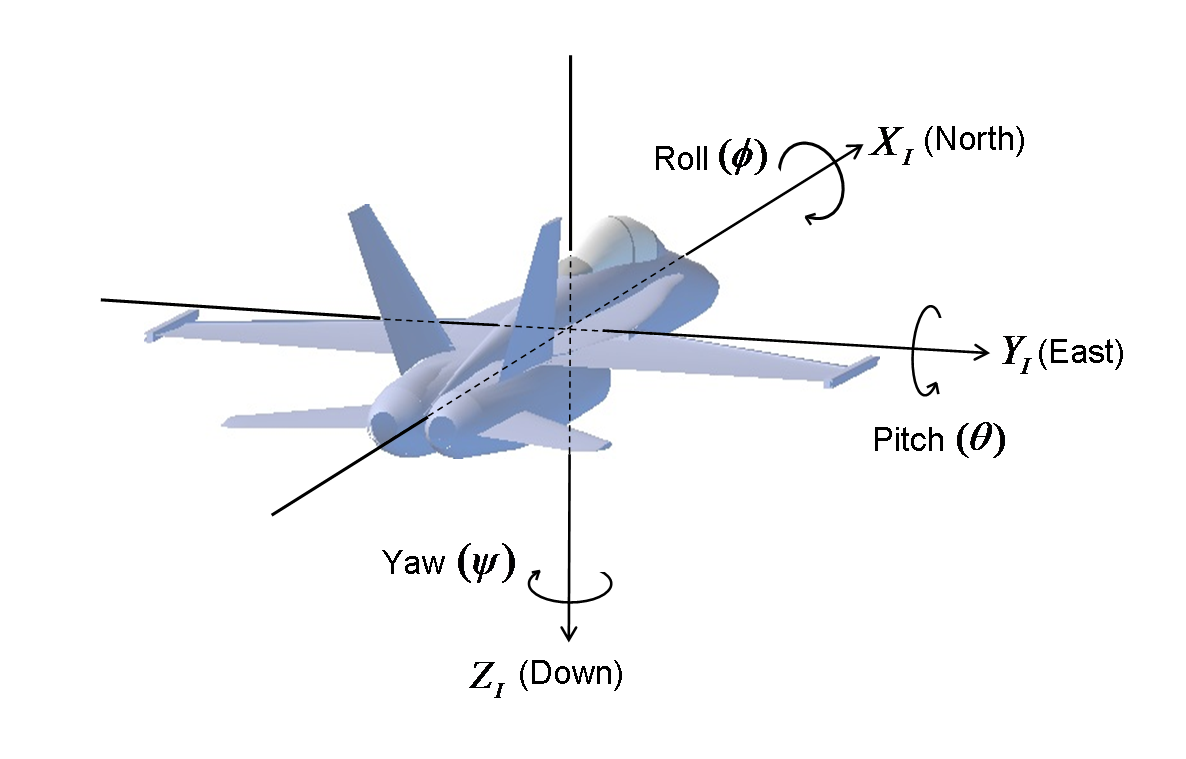
\includegraphics[width=\textwidth]{euler_aeroplane}
		\end{column}
	\end{columns}
\end{frame}

\begin{frame}{Representing look direction}
	\begin{columns}
		\pause
		\begin{column}{0.48\textwidth}
			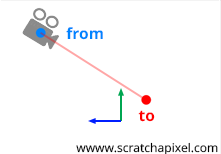
\includegraphics[width=\textwidth]{look_at}
		\end{column}
		\begin{column}{0.48\textwidth}
			\begin{itemize}
				\pause\item Don't need roll, just pitch and yaw to look up/down and left/right.
				\pause\item Eliminates the gimbal lock problem! :D
				\pause\item \textbf{Forward vector} / \textbf{look vector} can be obtained by appropriate rotation of a \textbf{unit vector}.
			\end{itemize}
		\end{column}
	\end{columns}
\end{frame}

\begin{frame}{Unit vectors}
	\begin{itemize}
		\pause\item A \textbf{unit vector} is a vector of length 1
		\pause\item I.e.\ $\sqrt{x^2 + y^2 + z^2} = 1$ (Pythagoras)
		\pause\item Useful to represent \textbf{direction}
		\pause\item Multiplying a vector of length $a$ by a number $b$ gives a vector of length $a \times b$,
			parallel to the original vector
		\pause\item So multiplying a unit vector by $b$ gives a vector of length $b$,
			parallel to the unit vector		
	\end{itemize}
\end{frame}

\begin{frame}{Moving forwards}
	\pause
	\begin{center}
		\colorbox{white}{
			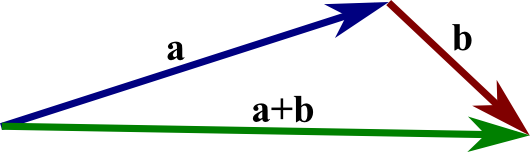
\includegraphics[width=0.5\textwidth]{vector_addition}
		}
	\end{center}
	\begin{itemize}
		\pause\item E.g.\ if $a$ is current position, and
		\pause\item $b$ is the distance and direction we want to move, then
		\pause\item $a + b$ is the new position
	\end{itemize}
\end{frame}

\begin{frame}{Addition in homogeneous coordinates}
	\begin{itemize}
		\pause\item Recall: homogeneous coordinates have an extra $w$ component, i.e.\ $(x,y,z,w)$
		\pause\item $w=1$ for positions, $w=0$ for offsets
	\end{itemize}
	\begin{tabular}{rclclc}
		\pause offset & + & offset & = & offset & $w = 0 + 0 = 0$ \\
		\pause position & + & offset & = & position & $w = 1 + 0 = 1$ \\
		\pause position & + & position & = & ??? & $w = 1 + 1 = 2$
	\end{tabular}
\end{frame}

